% ============================================================
% 电路基础实验 —— 实验三 等效电源定理 实验报告
% 使用 CircuitTheory/template.tex 正式实验报告模板
% ============================================================

\documentclass[12pt]{ctexart}

\usepackage{graphicx}
\usepackage{amsmath}
\usepackage{float}
\usepackage{booktabs}
\usepackage{siunitx}
\usepackage{caption}
\usepackage{subcaption}
\usepackage{enumitem}
\usepackage{fancyhdr}
\usepackage{hyperref}
\usepackage{makecell}

\sisetup{per-mode=symbol}

\graphicspath{{./figures/}{../}{../requirements/extracted_images/word/media/}{./}}

\usepackage[left=2.5cm, right=2.5cm, top=2.5cm, bottom=2.5cm]{geometry}

\setlength{\jot}{6pt}
\setlength{\headheight}{15pt}
\linespread{1.5}
\setlist{nosep}

\pagestyle{fancy}
\fancyhead[C]{电路基础实验}
\fancyfoot[C]{\thepage}

\begin{document}

\thispagestyle{empty}

\begin{figure}[t]
    \centering
    
\includegraphics[width=13cm]{logo1.png}
\end{figure}

\vspace*{\fill}
    \begin{center}
        \Huge\textbf{电路基础}

        \vspace{0.3cm}
        \Huge\textbf{实验报告}

        \vspace{1cm}
        \LARGE\textbf{实验三：等效电源定理}
    \end{center}
\vspace*{\fill}

\begin{table}[H]
    \centering
    \large
    \begin{tabular}{ll}
    \toprule
    \textbf{课程:} & 电路基础实验 \\
    \textbf{姓名:} & 郭浩然 2024303980 \\
    \textbf{组号:} & 第7组 \\
    \textbf{时间:} & \today \\
    \bottomrule
    \end{tabular}
\end{table}

\newpage

\section{实验目的}

\begin{enumerate}[label=\arabic*.]
    \item 学习并验证戴维南定理，理解线性有源单口网络对外等效的物理意义。
    \item 掌握等效电源内阻的测量方法，包括直接测量法、开路短路法、二次测量法和半偏法。
    \item 学习使用可调电阻作为负载，通过改变负载比较原电路与等效电路的端口伏安特性。
\end{enumerate}

\section{实验原理}

\subsection{戴维南定理}

戴维南定理指出，任意线性有源单口网络，从外部端口看，都可以等效为一个理想电压源与一个电阻串联的形式。理想电压源的电压等于原网络端口的开路电压，串联电阻等于原网络中所有独立源置零后从端口看进去的等效电阻。若端口电流按从等效电源流向负载方向取正，则端口电压与电流满足
\begin{equation}
    U = U_{oc} - I R_{\mathrm{th}},
\end{equation}
其中，\(U_{oc}\) 为开路电压，\(R_{\mathrm{th}}\) 为戴维南等效内阻，\(U\) 和 \(I\) 分别为外接负载时的端口电压和端口电流。

求取等效内阻时，需要将原网络中的独立源置零：理想电压源用短路代替，理想电流源用开路代替。若电路中含有受控源，则受控源不能置零，应保留其控制关系。

\subsection{等效内阻测量方法}

\subsubsection{直接测量法}

将被测有源网络中的独立电源置零后，从输出端口用万用表欧姆档直接测量等效电阻。该方法操作简单，但必须在电路断电状态下进行，且测量结果会受到连接状态和仪表内部测量方式的影响。

\subsubsection{开路短路法}

先测量端口开路时的电压 \(U_{oc}\)，再测量端口短路时的短路电流 \(I_{sc}\)。由戴维南等效电路可得
\begin{equation}
    R_{\mathrm{th}}=\frac{U_{oc}}{I_{sc}}.
\end{equation}
若 \(I_{sc}\) 以 \(\mathrm{mA}\) 为单位记录，计算电阻时应换算为安培：
\begin{equation}
    R_{\mathrm{th}}=\frac{U_{oc}}{I_{sc}\times 10^{-3}}.
\end{equation}

\subsubsection{二次测量法}

先测量端口开路电压 \(U_{oc}\)，再接入已知负载 \(R_L\)，测量负载端电压 \(U_L\)。根据分压关系有
\begin{equation}
    U_L = U_{oc}\frac{R_L}{R_{\mathrm{th}}+R_L},
\end{equation}
因此
\begin{equation}
    R_{\mathrm{th}}=R_L\left(\frac{U_{oc}}{U_L}-1\right).
\end{equation}
该方法不需要直接短接端口，适合用于不便测量短路电流的电路。

\subsubsection{半偏法}

对于戴维南等效电路，当负载电阻 \(R_L\) 等于等效内阻 \(R_{\mathrm{th}}\) 时，负载端电压为开路电压的一半：
\begin{equation}
    U_L=\frac{U_{oc}}{2}\quad\Longrightarrow\quad R_L=R_{\mathrm{th}}.
\end{equation}
因此可通过调节可变负载，使负载电压达到开路电压的一半，从而估算等效内阻。

\subsection{实验电路与 Multisim 仿真}

实验三的 Multisim 参考仿真电路如图~\ref{fig:thevenin-multisim} 所示。实验时先测量原线性有源网络的开路电压、短路电流和负载端口伏安特性，再根据测得的 \(U_{oc}\) 与 \(R_{\mathrm{th}}\) 搭建戴维南等效电路，最后比较两种电路在相同负载下的端口电压与电流。

\begin{figure}[H]
    \centering
    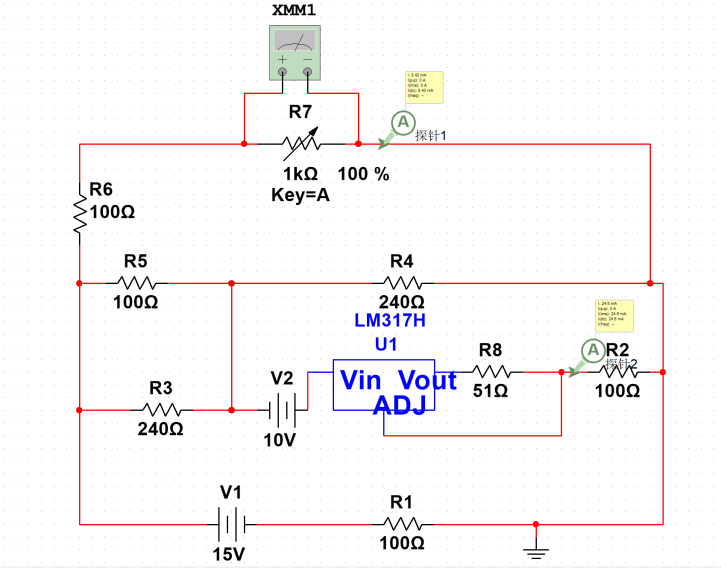
\includegraphics[width=0.82\textwidth]{image6.png}
    \caption{实验三 Multisim 参考仿真电路}
    \label{fig:thevenin-multisim}
\end{figure}

根据预习阶段的 Multisim 仿真结果，原网络端口开路电压和短路电流分别为
\begin{align}
    U_{oc} &= 9.909\,\mathrm{V}, \\
    I_{sc} &= 55.76\,\mathrm{mA}.
\end{align}
由开路短路法得到
\begin{equation}
    R_{\mathrm{th}}=\frac{9.909}{55.76\times 10^{-3}}\approx 177.71\,\Omega.
\end{equation}

\begin{table}[H]
    \centering
    \caption{原电路与戴维南等效电路仿真结果对比}
    \label{tab:simulation-result}
    \begin{tabular}{ccccc}
        \toprule
        负载电阻/\(\Omega\) & 原电路 \(U\)/V & 原电路 \(I\)/mA & 等效电路 \(U\)/V & 等效电路 \(I\)/mA \\
        \midrule
        100 & 3.620 & 36.30 & 3.545 & 35.52 \\
        510 & 7.352 & 14.42 & 7.325 & 14.42 \\
        1000 & 8.432 & 8.52 & 8.366 & 8.32 \\
        \bottomrule
    \end{tabular}
\end{table}

\section{实验器件}

\begin{itemize}
    \item 面包板 \(\times 1\)
    \item 可编程直流电源 \(\times 1\)
    \item 数字万用表 \(\times 1\)
    \item 电阻：\(51\,\Omega\times 1\)、\(100\,\Omega\times 4\)、\(240\,\Omega\times 2\)
    \item 可调电阻或可变负载 \(\times 1\)
    \item 导线若干
\end{itemize}

\section{实验步骤}

\begin{enumerate}[label=\arabic*.]
    \item 根据实验电路图选择所需电阻，在面包板上搭建原线性有源单口网络，并检查电源极性、公共节点和输出端口连接是否正确。
    \item 接入直流电源，测量原网络输出端口的开路电压 \(U_{oc}\)。
    \item 将输出端口短接并串入电流档，测量短路电流 \(I_{sc}\)，由开路短路法计算等效内阻 \(R_{\mathrm{th}}\)。
    \item 将独立电源置零后，从输出端口直接测量等效内阻，并与开路短路法的结果比较。
    \item 在原电路输出端接入可调负载，改变负载电阻，分别测量端口电压和负载电流。
    \item 根据测得的开路电压和等效内阻搭建戴维南等效电路，在等效电路输出端接入相同负载并测量端口电压和电流。
    \item 整理原电路与等效电路在不同负载下的测量数据，比较端口伏安特性并分析误差来源。
\end{enumerate}

\begin{figure}[H]
    \centering
    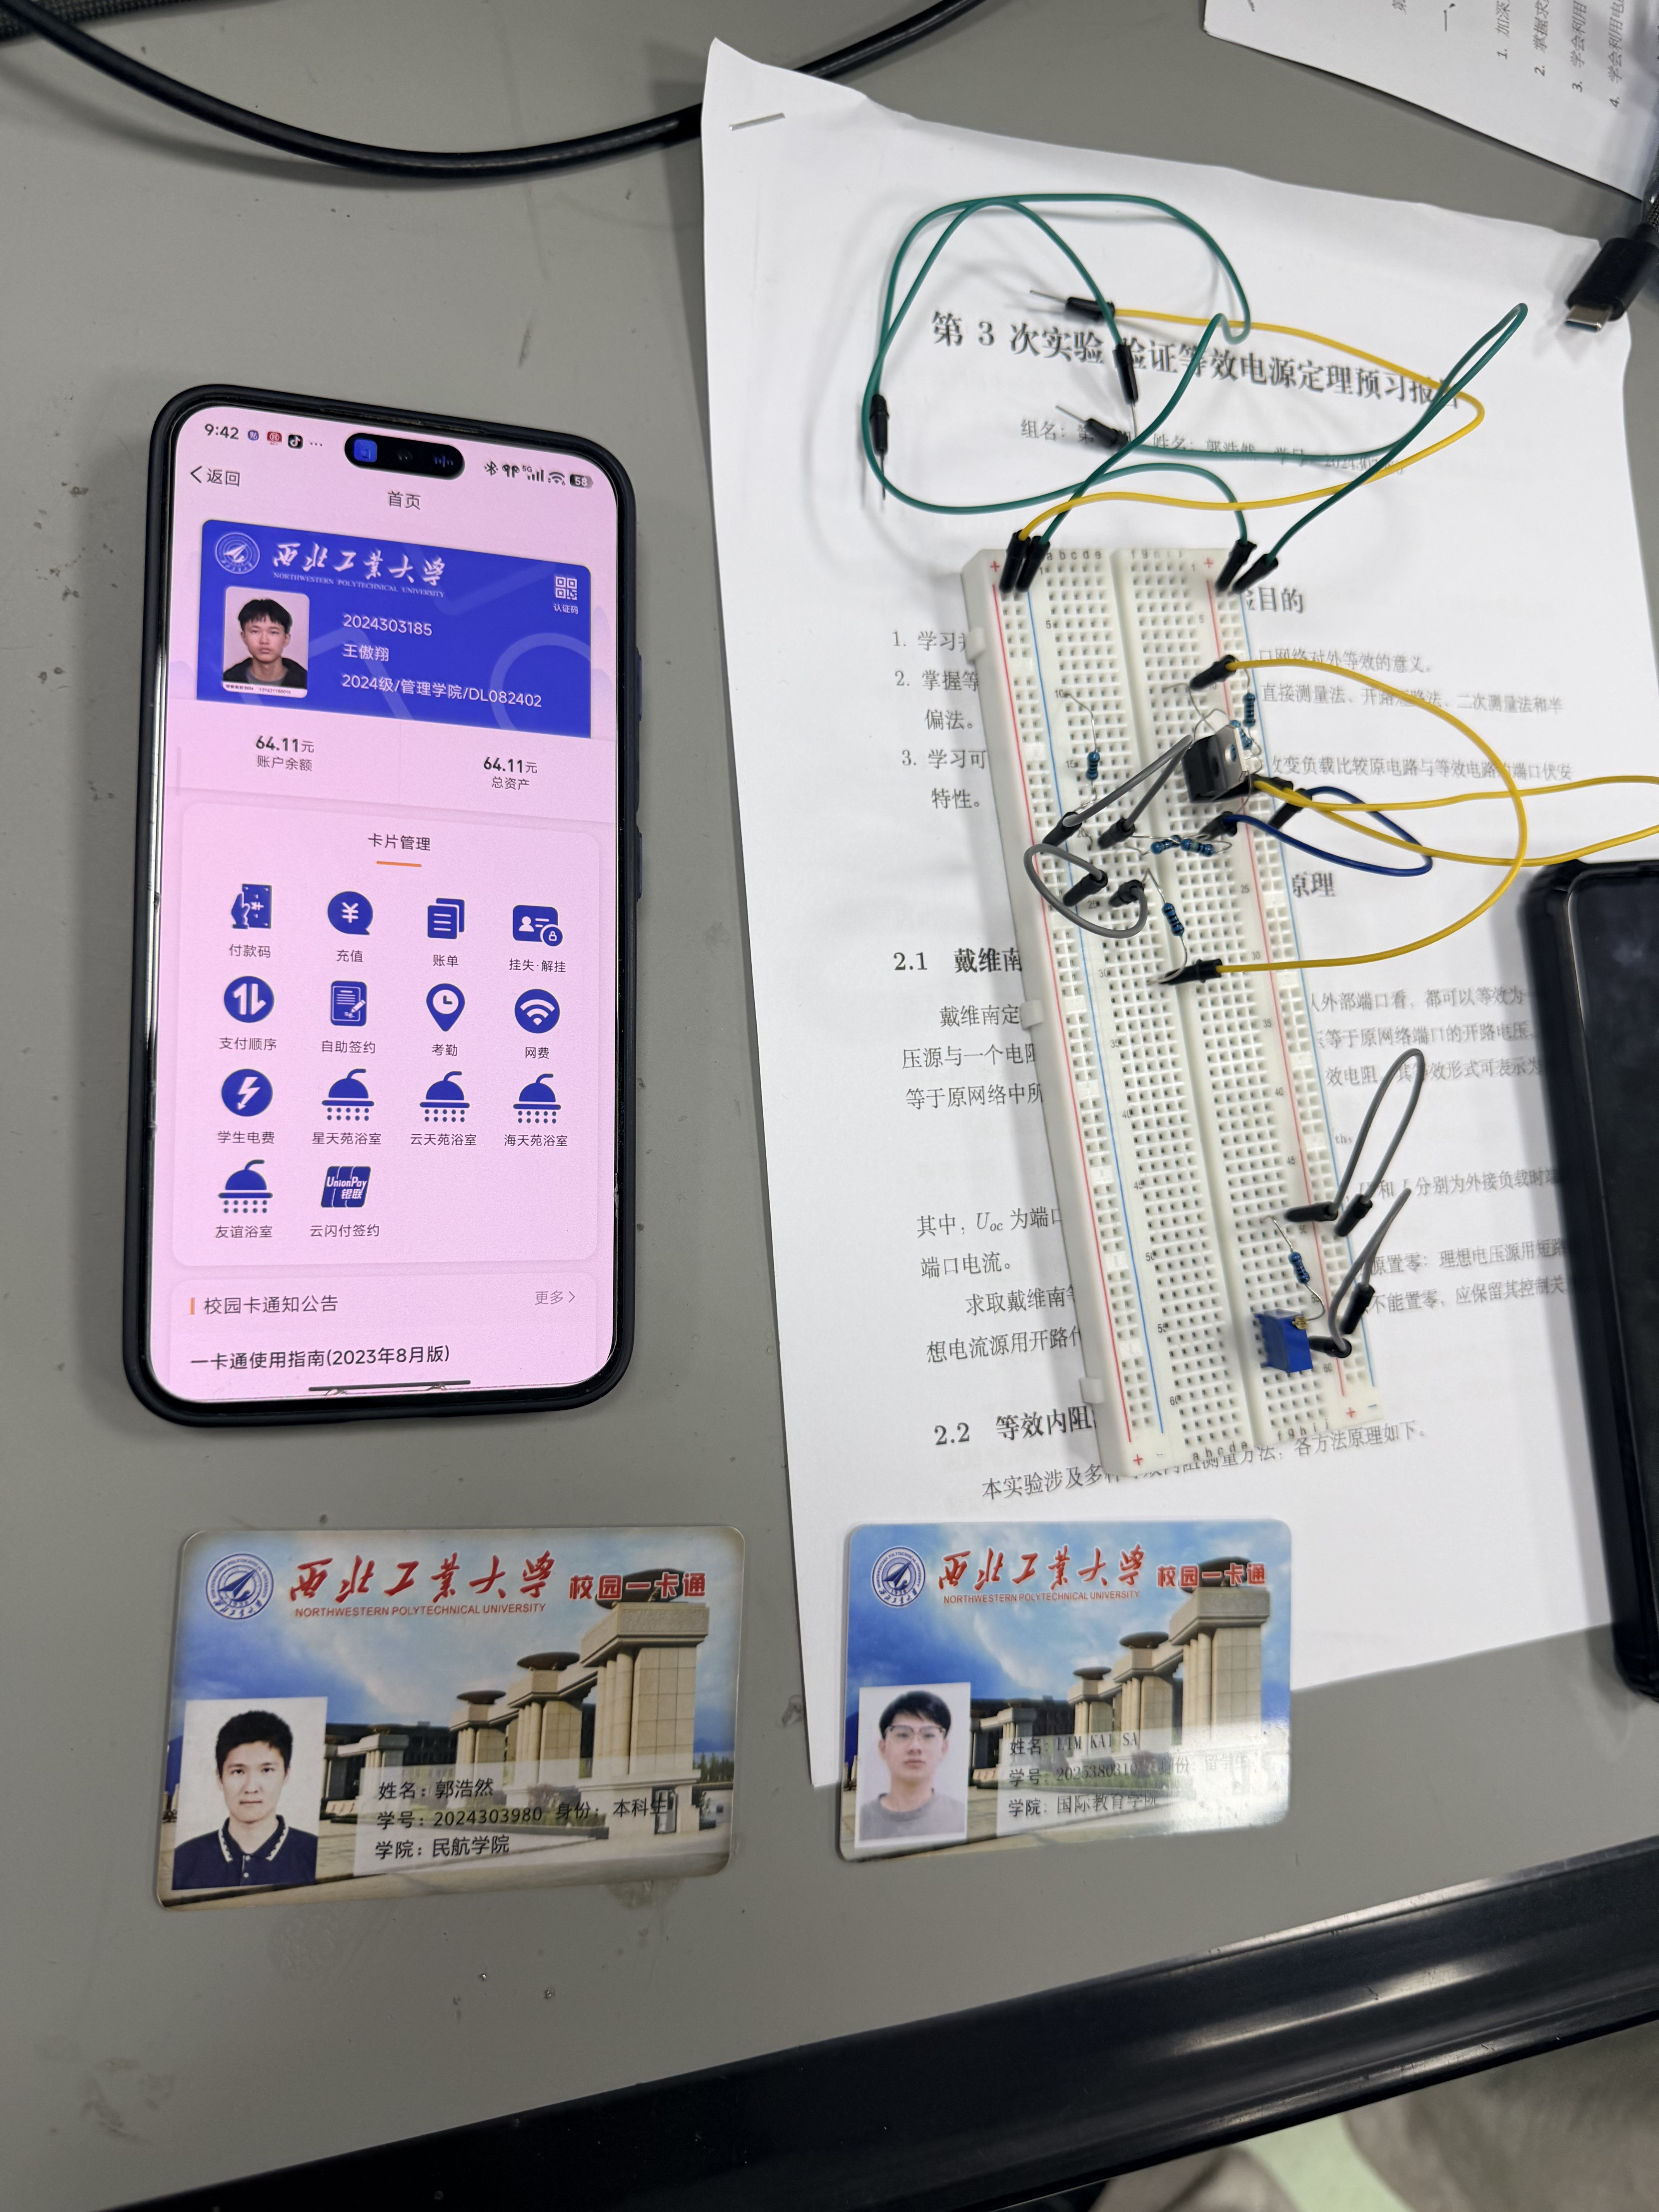
\includegraphics[width=0.82\textwidth]{physical_circuit_upright.jpg}
    \caption{实验三实物电路连接}
    \label{fig:physical-circuit}
\end{figure}

\section{实验数据}

实验原始数据记录如图~\ref{fig:raw-data} 所示。整理时仅录入原始记录中未被划掉且能够确定辨认的有效数据；被划掉的数据和未记录数据不作为有效实验数据使用。

\begin{figure}[H]
    \centering
    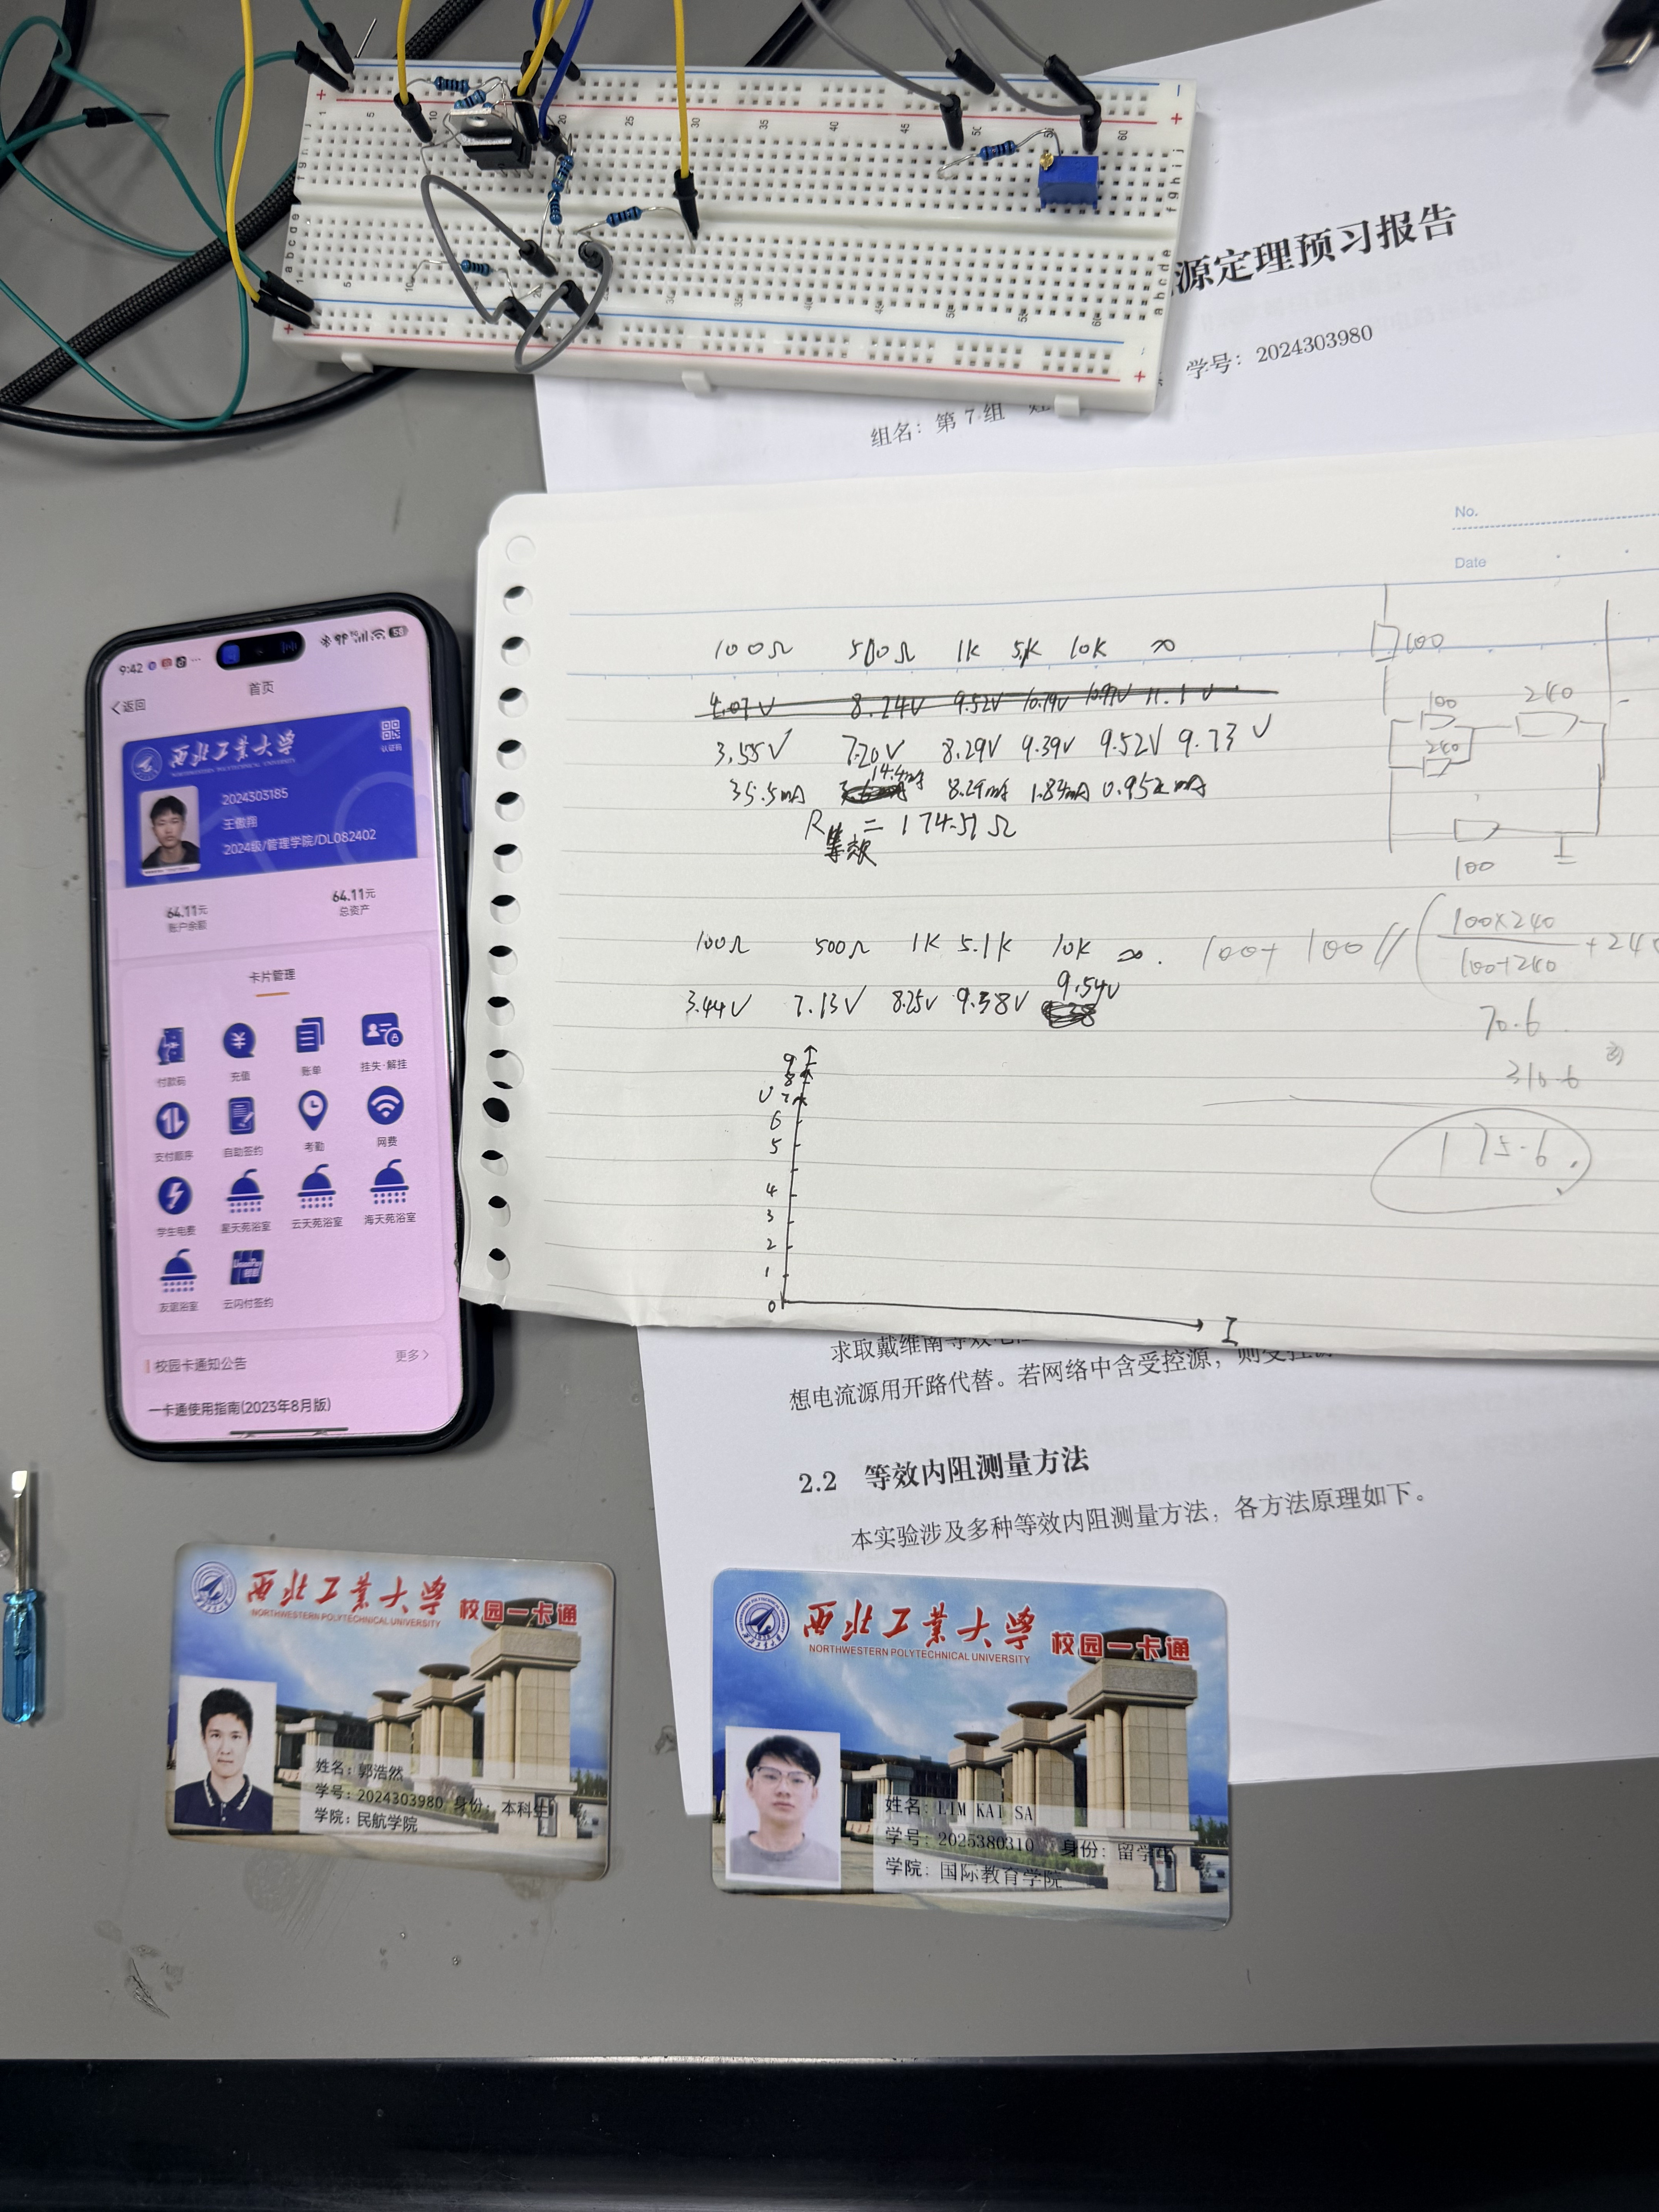
\includegraphics[width=0.82\textwidth]{raw_data_upright.jpg}
    \caption{实验三原始数据记录照片}
    \label{fig:raw-data}
\end{figure}

\begin{table}[H]
    \centering
    \caption{等效内阻测量数据整理}
    \label{tab:rth-measurement}
    \begin{tabular}{cccc}
        \toprule
        测量方法 & 测量量一 & 测量量二 & 等效内阻/\(\Omega\) \\
        \midrule
        直接测量法 & \(R=174.3\,\Omega\) & -- & 174.3 \\
        开路法 & \(U_{oc}=9.73\,\mathrm{V}\) & \(I=0\,\mathrm{mA}\) & -- \\
        \bottomrule
    \end{tabular}
\end{table}

\begin{table}[H]
    \centering
    \caption{原电路负载测量数据}
    \label{tab:original-load}
    \begin{tabular}{ccc}
        \toprule
        负载电阻/\(\Omega\) & 端口电压/V & 端口电流/mA \\
        \midrule
        100 & 3.55 & 35.5 \\
        500 & 7.20 & 14.4 \\
        1000 & 8.29 & 8.29 \\
        5100 & 9.39 & 1.84 \\
        10000 & 9.52 & 0.952 \\
        \(\infty\) & 9.73 & 0 \\
        \bottomrule
    \end{tabular}
\end{table}

\begin{table}[H]
    \centering
    \caption{戴维南等效电路负载测量数据}
    \label{tab:equivalent-load}
    \begin{tabular}{ccc}
        \toprule
        负载电阻/\(\Omega\) & 端口电压/V & 端口电流/mA \\
        \midrule
        100 & 3.44 & 34.4 \\
        500 & 7.13 & 14.26 \\
        1000 & 8.25 & 8.25 \\
        5100 & 9.38 & 1.84 \\
        10000 & 9.54 & 0.954 \\
        \bottomrule
    \end{tabular}
\end{table}

\begin{table}[H]
    \centering
    \caption{原电路与戴维南等效电路测量结果对比}
    \label{tab:load-comparison}
    \begin{tabular}{ccccccc}
        \toprule
        负载电阻/\(\Omega\) & 原电路 \(U\)/V & 等效电路 \(U\)/V & \(\Delta U\)/V & 原电路 \(I\)/mA & 等效电路 \(I\)/mA & \(\Delta I\)/mA \\
        \midrule
        100 & 3.55 & 3.44 & 0.11 & 35.5 & 34.4 & 1.10 \\
        500 & 7.20 & 7.13 & 0.07 & 14.4 & 14.26 & 0.14 \\
        1000 & 8.29 & 8.25 & 0.04 & 8.29 & 8.25 & 0.04 \\
        5100 & 9.39 & 9.38 & 0.01 & 1.84 & 1.84 & 0.00 \\
        10000 & 9.52 & 9.54 & 0.02 & 0.952 & 0.954 & 0.002 \\
        \bottomrule
    \end{tabular}
\end{table}

\section{数据分析}

\subsection{等效内阻测量结果分析}

等效内阻可由直接测量法、开路短路法、二次测量法和半偏法得到。本次原始记录中可确定读出的直接测量法结果为
\begin{equation}
    R_{\mathrm{th}}=174.3\,\Omega.
\end{equation}
同时，原电路开路时端口电压为 \(U_{oc}=9.73\,\mathrm{V}\)。若使用开路短路法，则计算公式为
\begin{equation}
    R_{\mathrm{th}}=\frac{U_{oc}}{I_{sc}\times 10^{-3}},
\end{equation}
其中 \(I_{sc}\) 的单位为 \(\mathrm{mA}\)。由于原始有效记录中未明确保留短路电流读数，表~\ref{tab:rth-measurement} 中主要采用直接测量法得到的等效内阻。该结果与预习仿真得到的 \(177.71\,\Omega\) 接近，相对偏差为
\begin{equation}
    \frac{|174.3-177.71|}{177.71}\times100\% \approx 1.92\%,
\end{equation}
说明实测等效内阻与仿真参考值吻合较好。

\subsection{原电路与等效电路端口特性比较}

戴维南定理要求原线性有源单口网络与其等效电路在外部端口表现出相同的伏安特性。根据式
\begin{equation}
    U = U_{oc} - I R_{\mathrm{th}},
\end{equation}
若以端口电流为横轴、端口电压为纵轴，则理论上两种电路的 \(U-I\) 关系应接近同一直线，其截距为 \(U_{oc}\)，斜率为 \(-R_{\mathrm{th}}\)。

由表~\ref{tab:load-comparison} 可知，当负载电阻分别为 \(100\,\Omega\)、\(500\,\Omega\)、\(1\,\mathrm{k}\Omega\)、\(5.1\,\mathrm{k}\Omega\) 和 \(10\,\mathrm{k}\Omega\) 时，原电路与戴维南等效电路的端口电压差分别为 \(0.11\,\mathrm{V}\)、\(0.07\,\mathrm{V}\)、\(0.04\,\mathrm{V}\)、\(0.01\,\mathrm{V}\) 和 \(0.02\,\mathrm{V}\)，电流差分别为 \(1.10\,\mathrm{mA}\)、\(0.14\,\mathrm{mA}\)、\(0.04\,\mathrm{mA}\)、\(0.00\,\mathrm{mA}\) 和 \(0.002\,\mathrm{mA}\)。除小负载下电流较大、绝对误差略明显外，其余负载点的电压和电流偏差均较小。

随着负载电阻增大，端口电压由约 \(3.55\,\mathrm{V}\) 升高到接近开路电压 \(9.73\,\mathrm{V}\)，端口电流由 \(35.5\,\mathrm{mA}\) 降低到接近零，变化趋势符合戴维南等效电路的分压关系。原电路与等效电路在相同负载下的端口电压、电流基本一致，说明戴维南等效电路能够在外部端口处较好地替代原线性有源网络。

\subsection{误差来源分析}

实验误差主要来自以下方面：
\begin{enumerate}[label=\arabic*.]
    \item 电阻实际阻值与标称阻值存在偏差，导致理论等效内阻和实际端口特性不完全一致。
    \item 可调电阻的实际阻值可能随旋钮位置和接触状态变化，读数稳定性有限。
    \item 数字万用表存在分辨率误差，电压、电流和电阻读数均可能出现小幅波动。
    \item 面包板、导线和接触点存在接触电阻，端口连接状态会影响电压和电流测量。
    \item 测量短路电流或串入电流档时，万用表内阻和接线方式会对原电路状态产生扰动。
    \item 直流电源实际输出电压可能与设定值存在微小差异。
\end{enumerate}

综上，直接测量得到的等效内阻与仿真参考值接近，原电路和戴维南等效电路在相同负载下的端口电压、电流也基本一致。实验结果表明，在实验误差允许范围内，戴维南等效电路能够从外部端口处替代原线性有源网络，等效电源定理得到验证。

\end{document}
